\subsubsection{Die Hardware-API}

Dieser Abschnitt erklärt den Teil der Hardware-Komponente, der für die Kommunikation mit der
Services-Komponente sowie für die Ansteuerung des Buttons und der LEDs zuständig ist.
Für diese Aufgabe war Manuel Radatz verantwortlich.

Wir haben uns dafür entschieden, dass die Hardware-Komponente und die Services-Komponente jeweils
verschiedene Programme darstellen.
Auf jeden Client laufen daher die Prozesse \texttt{services-client} und \texttt{hardware-api}.
Die Kommunikation erfolgt somit \textit{nicht} beispielsweise dadurch, dass von der
Services-Komponente eine Bibliothek verwendet wird, die die Hardware-Komponente bereitstellt,
sondern über Unix-Sockets.
Dabei werden Strings im Format von Google Protocol Buffers übertragen, denen jeweils ein Header mit
Nachrichten-ID und Nachrichtenlänge vorangestellt ist.
Durch die Verwendung von Protocol Buffers ist es möglich, dass die verschiedenen Komponenten in
unterschiedliche Programmiersprachen geschrieben werden können.
Dieser Flexibilität und einer besseren Wartbarkeit, die neben religiösen Gründen die Anlässe für
die Verwendung von Unix-Sockets und Google Protocol Buffers waren, stehen auf der anderen Seite ein
größerer Kommunikationsoverhead gegenüber.
Wegen der Rechenleistung der Raspberry Pis fällt dieser Overhead kaum ins Gewicht.
Da wir die gewonnene Flexibilität jedoch nicht genutzt haben und beide Komponenten in C++14
geschrieben sind, ist der Overhead letztendlich unnötig.
Rückblickend wäre es auch einfacher gewesen, wenn die Hardware-Komponente auf den Clients direkt
mit der Services-Komponente auf dem Server kommuniziert hätte, da wir uns später für eine
Client-Server-Architektur entschieden hatten.
Würde man das Projekt noch weiterentwickeln, könnte die jetzige Architektur allerdings noch von
Vorteil sein.

Die Hardware-API besteht aus dem in C++14 geschriebenen Programm \texttt{hardware-api}, das auf
allen Clients, jedoch nicht auf dem Server läuft.
C++ war für diese Aufgabe sehr gut geeignet.
Die Sprache hat einen sehr geringen Overhead und bietet die notwendige Flexibilität.
Hauptsächlich erfolgte diese Entscheidung jedoch wegen bereits vorhandenen Programmierkenntnissen
in dieser Sprache.
Die Entscheidung für die Version C++14 beruht darauf, dass dies die höchste Version ist, die von der
GCC-Version, die Raspbian zur Verfügung stellt, unterstützt wird.

Die API kommuniziert nach oben mit \texttt{services-client} über Unix-Sockets und Protocol Buffers.
Nach unten kommuniziert sie mit dem Infrarot-Treiber, indem dessen Quellcode bei der Kompilierung
der \texttt{hardware-api} direkt eingebunden wird, und sie spricht die LEDs und den Button direkt
über wiringPi an.

Für die Kommunikation nach oben wird die Socket-API der POSIX-C-Bibliothek genutzt.
Für die Einbettung in C++ und die Nutzbarkeit nach dem in dieser Sprache üblichen RAII-Prinzip
wurden für die Unix-Sockets die Wrapperklassen \texttt{CSocketWrapper}, \texttt{UnixReceiver} und
\texttt{UnixSender} geschrieben, die die Kommunikation über die Socket-API abstrahieren.
Dazu gehört auch das Puffern von unvollständigen empfangenen Nachrichten.
Außerdem dient die Klasse \texttt{FileDeleter} dazu, dass die für die Kommunikation über
Unix-Sockets notwendigen Dateien nach dem Beenden des Programms implizit gelöscht werden.
Die Klassen \texttt{TCPConnection}, \texttt{TCPServer} und \texttt{TCPClient} erfüllen dieselbe
Aufgabe für die TCP-Kommunikation, die für die später beschriebenen Testprogramme
\hyperref[client-stub-und-server-stub]{\texttt{client-stub} und \texttt{server-stub}} notwendig ist.
Alternativ hätte man auch bestehende Bibliotheken wie boost verwenden können, die ebenfalls eine
C++-Schnittstelle für die Netzwerkkommunikation zur Verfügung gestellt hätten.
Dafür hätte man sich zuerst in diese Bibliothek einarbeiten müssen und da Manuel Radatz, der diese
Komponente geschrieben hat, bereits Erfahrungen mit der C-Socket-API hatte, wäre das aufwendiger
gewesen als die Implementierung der Wrapperklassen, weshalb sie am Ende nicht genutzt wurde.
Da diese Wrapperklassen am Ende stabil liefen, war diese Entscheidung auch richtig.

Eine weitere Klasse (\texttt{InterfaceToServices}) abstrahiert die Kommunikation mit
\texttt{services-client}.
Sie ist hauptsächlich dafür zuständig, dass diese Kommunikation stabil bleibt und nach einem
Verbindungsabbruch (z.B. wenn \texttt{services-client} abgestürzt ist oder zu Testzwecken beendet
wird) wieder hergestellt wird.
Bei dem Empfangen von Nachrichten werden die zuvor von der \texttt{main()}-Funktion gesetzten
Callback-Funktionen aufgerufen.

Für die LED-Ansteuerung empfängt die Hardware-API von \texttt{services-client} Nachrichten, in denen
mit drei ganzen Zahlen kodiert ist, welches Ereignis wann und wie lange angezeigt werden soll.
Die Ereignisse, die übertragen werden, sind:
\begin{itemize}
  \item
    Spieler wurde getroffen und ist unverwundbar – mit der Information, wie lange der Spieler
    unverwundbar ist
  \item
    Spieler hat einen anderen Spieler getroffen – optional mit der Information, wie lange das dem
    Spieler angezeigt werden soll
  \item
    Spiel startet – mit der Information, wann das Spiel startet und wie lange das Spiel läuft
  \item
    Spiel endet – mit der Information, wann
  \item
    Spieler tot
  \item
    letztes Leben
\end{itemize}
Nicht alle Ereignisse werden in allen Spielmodi genutzt.
So gibt es beispielsweise Spielmodi, in denen es das Konzept von „Leben“ nicht gibt.
Das Ereignis „Spiel endet“ ist auch nur dann notwendig, wenn bei dem Ereignis „Spiel startet“ nicht
übertragen wurde, wie lange das Spiel läuft.

\phantomsection\label{led-anzeige}
\begin{figure}
  \centering
  \begin{subfigure}[b]{0.29\textwidth}
    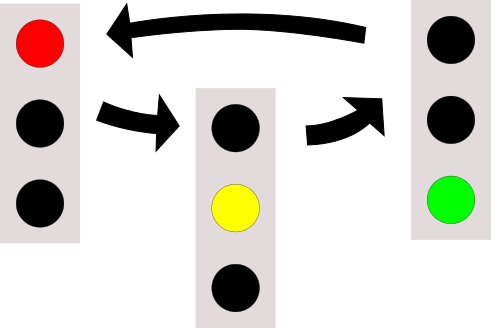
\includegraphics[width=\textwidth,keepaspectratio]
                    {./040-komponenten/010-hardware/led-default.png}
    \caption{\label{fig:led-init}}
  \end{subfigure}
  \hspace{0.1\textwidth}
  \begin{subfigure}[b]{0.46\textwidth}
    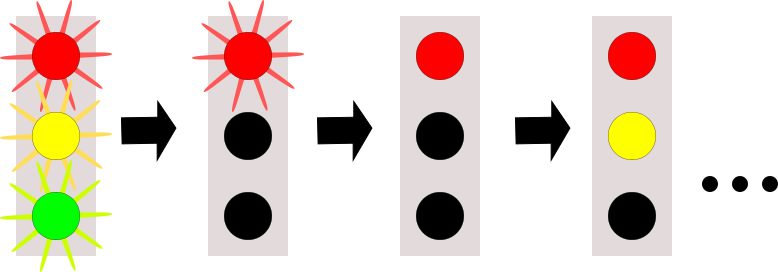
\includegraphics[width=\textwidth,keepaspectratio]{./040-komponenten/010-hardware/led-start.png}
    \caption{\label{fig:led-start}}
  \end{subfigure}
  
  \begin{subfigure}[b]{0.08\textwidth}
    
\includegraphics[width=\textwidth,keepaspectratio]{./040-komponenten/010-hardware/led-green.png}
    \caption{\label{fig:led-green}}
  \end{subfigure}
  \hspace{0.03\textwidth}
  \begin{subfigure}[b]{0.08\textwidth}
    
\includegraphics[width=\textwidth,keepaspectratio]
                    {./040-komponenten/010-hardware/led-green-blink.png}
    \caption{\label{fig:led-green-blink}}
  \end{subfigure}
  \hspace{0.03\textwidth}
  \begin{subfigure}[b]{0.08\textwidth}
    
\includegraphics[width=\textwidth,keepaspectratio]
                    {./040-komponenten/010-hardware/led-red-blink.png}
    \caption{\label{fig:led-red-blink}}
  \end{subfigure}
  \hspace{0.03\textwidth}
  \begin{subfigure}[b]{0.08\textwidth}
    
\includegraphics[width=\textwidth,keepaspectratio]{./040-komponenten/010-hardware/led-red.png}
    \caption{\label{fig:led-red}}
  \end{subfigure}
  \hspace{0.03\textwidth}
  \begin{subfigure}[b]{0.08\textwidth}
    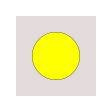
\includegraphics[width=\textwidth,keepaspectratio]
                    {./040-komponenten/010-hardware/led-yellow.png}
    \caption{\label{fig:led-yellow}}
  \end{subfigure}
  \hspace{0.03\textwidth}
  \begin{subfigure}[b]{0.08\textwidth}
    
\includegraphics[width=\textwidth,keepaspectratio]
                    {./040-komponenten/010-hardware/led-red-yellow-blink.png}
    \caption{\label{fig:led-red-yellow-blink}}
  \end{subfigure}
  \caption{LED-Zustände \\ \small
           \textbf{(\subref*{fig:led-init})} Initialer Zustand
           \textbf{(\subref*{fig:led-start})} Spielstart
           \textbf{(\subref*{fig:led-green})} Spiel läuft
           \textbf{(\subref*{fig:led-green-blink})} Spielende naht \\
           \textbf{(\subref*{fig:led-red-blink})} wurde getroffen (unverwundbar)
           \textbf{(\subref*{fig:led-red})} tot
           \textbf{(\subref*{fig:led-yellow})} hat getroffen
           \textbf{(\subref*{fig:led-red-yellow-blink})} letztes Leben}
  \label{fig:leds}
\end{figure}
Jedes Spielgerät hat jeweils eine rote, eine gelbe und eine grüne LED, die wie auf einer Ampel
angeordnet sind.
Für Menschen mit Rot-Grün-Schwäche könnte man auch Prototypen bauen, bei denen die grüne LED durch
eine blaue LED ersetzt wird.
Mit diesen LEDs werden die verschiedenen Ereignisse kodiert.
Läuft kein Spiel und ist auch kein Spiel angekündigt, so leuchten alle LEDs der Reihe nach auf.
Dadurch können defekte, sowie nicht- oder falsch-angeschlossene LEDs schon direkt nach dem
Einschalten der Spielgeräte erkannt werden.
Wird ein Spiel angekündigt, so fangen alle LEDs synchron an zu blinken.
10 Sekunden vor dem Spielstart blinkt dann nur noch die rote LED und 4 Sekunden davor schalten die
LEDs, analog zu einer deutschen Ampel, von rot über rot-gelb auf grün.
Die grüne LED zeigt an, dass das Spiel läuft.
Neigt sich das Spiel dem Ende zu, fängt die grüne LED 64 Sekunden vorher langsam an zu blinken und
blinkt bis zum Ende des Spiels immer schneller.
Nach dem Spielende kehren die LEDs zum initialen Zustand zurück.
Wenn das Spiel läuft, zeigt das Blinken der roten LED an, dass man getroffen wurde und unverwundbar
ist.
Auch sie wird immer schneller, wenn die Zeit der Unverwundbarkeit abläuft.
Zeigt die LED Dauerrot, dann ist man tot.
In diesem Zustand ist es auch nicht mehr möglich, andere Spieler abzuschießen, d.h. der IR-Sender
wird deaktiviert.
Die gelbe LED zeigt an, dass man einen anderen Spieler getroffen hat.
Das letzte Leben wird dadurch angezeigt, dass die rote und die gelbe LED etwa alle 2 Sekunden für
100 Millisekunden synchron aufleuchten.
Alle LED-Zustände sind zur Übersicht auch in \cref{fig:leds} dargestellt.

Ursprünglich wollten wir anstelle von LEDs ganze Displays verwenden, um auch individuelle
Informationen als Text oder eine Karte des Spielfeldes mit allen Mitspielern anzeigen zu können.
Neben des begrenzten Budgets und der Tatsache, dass Informationen dieser Art auch auf der Webseite
angezeigt werden können, war auch die begrenzte Zeit ein Grund dafür, dass wir diese Idee verworfen
haben.
Auch die Karte wurde nicht umgesetzt, da für die zuverlässige und genaue Positionsermittlung eines
Spielers in geschlossenen Räumen diverse Probleme zeit- und kostenintensiv gelöst werden müssten und
dies jenseits unserer Möglichkeiten in diesem Projekt gewesen wäre.
(Trotzdem wurde zunächst viel Zeit in diese Idee investiert.)

Die LED-Ansteuerung erfolgt ebenfalls in einer eigenen Klasse namens \texttt{LEDEventStatus}.
Diese ruft direkt Funktionen von wiringPi auf, verwaltet alle Daten, die zur korrekten
LED-Ansteuerung notwendig sind (auch die Timer) und interpretiert als Eingabe das von
\texttt{services-client} empfangene Zahlentripel.

Der Status des Buttons wird direkt in der \texttt{main()}-Funktion durch Aufrufe der
wiringPi-Funktionen abgefragt.

Die \texttt{main()}-Funktion besteht abgesehen von der Initialisierung aus einer Schleife, die erst
dann verlassen wird, wenn das Programm \texttt{SIGTERM} empfängt oder eine Exception auftritt, die
auf größere Probleme hindeutet.
Dort besteht jede Iteration aus:
\begin{itemize}
  \item
    das Abfragen, ob Nachrichten von \texttt{services-client} angekommen sind, welche dann auch
    durch das Aufrufen von Callback-Funktionen interpretiert werden,
  \item
    die Aktualisierung des LED-Status,
  \item
    die Abfrage des Buttons, ob dieser gedrückt wird, wobei in diesem Fall die eigene Client-ID an
    den IR-Sender gesendet wird und
  \item
    das Abfragen des IR-Sensors, ob Daten empfangen wurden sowie die Weiterleitung dieser an
    \texttt{services-client}.
\end{itemize}
Danach wartet das Programm 0,5 Millisekunden, um die CPU-Auslastung gering und folglich die
Temperatur des Prozessors niedrig zu halten und die Lebensdauer des Akkumulators zu erhöhen.
Die dadurch entstehende Latenz von bis zu 0,5 Millisekunden ist so niedrig, dass sie keine spürbaren
Auswirkungen auf das Spiel haben sollte.
Wird der Button gedrückt, werden auch nicht in jeder Iteration IR-Daten gesendet.
Dies würde zu einer Überbeanspruchung der IR-LED führen.
Stattdessen werden ab dem Moment, in dem der Button heruntergedrückt wird, nur alle 100
Millisekunden IR-Daten an den IR-Treiber übergeben.

Neben diesem regulären Ablauf wurden auch zahlreiche Features zum Testen implementiert, welche über
Programmparameter ein- oder ausgeschaltet werden können.
Ist kein Button vorhanden, so besteht die Möglichkeit, dass ohne Unterbrechung alle 500
Millisekunden die eigene Client-ID an den IR-Sender gesendet wird.
Wenn kein IR-Empfänger funktionsfähig ist, das Programm auf anderer Hardware ausgeführt wird oder
nur die Kommunikation mit \texttt{services-client} getestet werden soll, gibt es zusätzlich einen
automatischen und einen manuellen Testmodus.
Im automatischen Testmodus werden regelmäßig zufällige Daten an \texttt{services-client} gesendet,
als wären diese von dem IR-Sensor empfangen worden.
Im manuellen Testmodus kann man manuell Testdaten eingeben, die gesendet werden sollen.
In beiden Testmodi wird der LED-Status auch auf der Konsole ausgegeben.
Dadurch sind Tests auch ziemlich einfach in virtuellen Umgebungen ohne die Hardware möglich.

\phantomsection\label{client-stub-und-server-stub}
Außerdem wurden Stubs implementiert, welche \texttt{services-client} ersetzen können, sodass auch
andersherum die Hardware ohne Services getestet oder demonstriert werden kann.
Dazu gehört der Stub \texttt{led-trigger}, mit dem man manuell LED-Ereignisse an die
\texttt{hardware-api} senden kann, sowie das Paar von Stubs \texttt{client-stub} und
\texttt{server-stub}, von denen einer auf den Clients und einer auf dem Server läuft, der alle
empfangenen IR-Daten in Echtzeit auf dem Server ausgibt, was das ansonsten erforderliche
Nachschauen in Log-Dateien beim Debuggen erspart.

Das Programm \texttt{hardware-api} läuft im fertigen System als Daemon.
Es kann aber auch als gewöhnliches Programm gestartet werden, was zum interaktiven Testen auch
notwendig ist.

Der build-Prozess erfolgt durch eine einzige Makefile.
Wegen der Einfachheit des Programms und der Tatsache, dass die Programme gezielt für ein bestimmtes
System entwickelt worden sind, wäre die Nutzung von cmake oder des GNU Build Systems überflüssig
gewesen.
